\documentclass[13pt]{beamer}
% \usecolortheme{whale}
\usetheme{Boadilla}
\usecolortheme{seahorse}
% \usetheme{Singapore}
\usepackage{lipsum}
\usepackage{fancybox}
% \usepackage{fontspec}
\usepackage{xeCJK}
\setCJKmainfont[AutoFakeBold=true]{TW-Sung}
% \setCJKsansfont{Kurier}

\setbeamertemplate{navigation symbols}{}

\usepackage{tabto}
\usepackage{parskip}  % No-indent
% \usepackage{enumitem} % change enumerate behaviours
\usepackage{lipsum} %
\usepackage{color}
\usepackage{siunitx}
\usepackage{newclude} %make include only not clearpage
\usepackage{multicol}
\setlength{\fboxsep}{0.6em}
\usepackage{graphics}
\usepackage{tabularx}
\usepackage{tcolorbox}
\usepackage{makecell}
\usepackage{tikz}
\usetikzlibrary{positioning}
%Information to be included in the title page:
\title{第一課}
\author{波的基本性質}
\institute{}
\date{}

% \setbeamerfont{normal text}{size=\HUGE}
% \setbeamerfont{block title}{size=\HUGE}

\newcounter{saveenumi}
\newcommand{\seti}{\setcounter{saveenumi}{\value{enumi}}}
\newcommand{\conti}{\setcounter{enumi}{\value{saveenumi}}}


\newcommand{\shc}[1]{
    \qty[mode = text]{#1}{J.kg^{-1}.\degreeCelsius^{-1}}
}
\newcommand{\hc}[1]{
    \qty[mode = text]{#1}{J.\degreeCelsius^{-1}}
}
\newcommand{\oc}[1]{
\qty{#1}{\degreeCelsius}
}
\newcommand{\slh}[1]{\qty{#1}{J.kg^{-1}}}




\begin{document}
\frame{\titlepage}


% \fontsize{<size>}{<vskip>}\selectfont % set fontsize and vskip of a frame

\section{oscillation}

\begin{frame}{振動的典型例子}
    \begin{columns}
        \column{.5\textwidth}
        \begin{figure}
            \centering
            \includegraphics[width=0.5\linewidth]{images/Screenshot 2023-09-24 at 8.42.59 PM.png}
            \caption{鐘擺}

        \end{figure}
        \column{.5\textwidth}
        \begin{figure}
            \centering
            \includegraphics[width=0.5\linewidth]{images/Screenshot 2023-09-24 at 8.43.04 PM.png}
            \caption{負重彈簧}

        \end{figure}
    \end{columns}
\end{frame}

\begin{frame}{振動}
    \begin{itemize}
        \item 振動過程中圍繞着一個\textbf{平衡位置}進行週期性運動。
        \item 在平衡位置中,物件的速率是最大值。
        \item 振動過程中也存在兩個極端位置,當中物件是\textbf{瞬時靜止}。
    \end{itemize}
\end{frame}

\begin{frame}{振動}
    \begin{figure}
        \centering
        \includegraphics[width=.9\linewidth]{images/Screenshot 2023-09-24 at 8.52.36 PM.png}


    \end{figure}
\end{frame}


\begin{frame}{波動的特性}
    \begin{itemize}
        \item 波動是一種能量的傳播形式。
        \item 對於\textbf{機械波}來說,波動的傳播需要\textbf{介質}。
        \item \textbf{機械波}包括:
              \begin{itemize}
                  \item 彈簧上的波
                  \item 水波
                  \item 聲波
                  \item 地震波
              \end{itemize}
        \item 另一種波是\textbf{電磁波},不是機械波,因為不需要介質來傳播。
    \end{itemize}
\end{frame}

\begin{frame}{波動的特性}
    \begin{figure}
        \centering
        \includegraphics[width=0.75\linewidth]{images/Screenshot 2023-09-24 at 9.06.45 PM.png}
        \caption{介質中的質點進行振動,構成了機械波}

    \end{figure}
\end{frame}

\begin{frame}{不同的波傳播的能量}
    \begin{itemize}
        \item 太陽能通過可見光波傳播到地球。
        \item 聲音通過空氣中的聲波傳遞到我們的耳朵。
        \item 能量透過水面上的水波傳遞。
        \item 能量在地震中透過地震波傳遞。

    \end{itemize}
\end{frame}

\begin{frame}{脈衝}

    \begin{itemize}
        \item 脈衝是一個持續短暫時間的波。
        \item 如果給一條繩子一股脈衝,它會以固定的速率在繩子上移動。
    \end{itemize}
    \bigskip
    \begin{figure}
        \centering
        \includegraphics[width=1\linewidth]{images/Screenshot 2023-09-24 at 9.19.05 PM.png}


    \end{figure}
\end{frame}

\begin{frame}{波的種類}
    \begin{alertblock}{橫波}
        (質點)振動的方向\textbf{垂直}於波動傳播的方向。
    \end{alertblock}
    \begin{alertblock}{縱波}
        (質點)振動的方向\textbf{平行}於波動傳播的方向。
    \end{alertblock}
    \begin{itemize}
        \item 機械波可以是橫波或縱波。
        \item 電磁波只能是橫波。
    \end{itemize}
\end{frame}

\begin{frame}{波的例子}
    \begin{columns}
        \column{.45\textwidth}


        \begin{exampleblock}
            {橫波的例子:}
            \begin{itemize}
                \item 水波
                \item 繩子上的波
                \item 光波
                \item 無線電波
                \item 微波
                \item 紅外輻射
                \item 紫外輻射
                \item X射線
                \item 伽碼射線
            \end{itemize}
        \end{exampleblock}
        \column{.45\textwidth}
        \begin{exampleblock}
            {縱波的例子:}
            \begin{itemize}
                \item 彈簧上的波
                \item 聲波
                \item 超聲波
            \end{itemize}
        \end{exampleblock}

    \end{columns}


\end{frame}

% \begin{frame}{波的特徵}
%     \begin{itemize}
%         \item 當波通過介質傳播時,每個質點都會在其平衡位置周圍進行振動。
%         \item 每個質點\textbf{距離其平衡位置的距離}稱為\textbf{位移} y。
%         \item 波的\textbf{振幅} A 是質點距離平衡位置的\textbf{最大位移}。
%         \item 振幅與波的能量或強度有關。
%         \begin{itemize}
%             \item 振幅較大的波盛載較多的能量。
%         \end{itemize}
%     \end{itemize}
%     \bigskip
%     \begin{figure}
%         \centering
%         \includegraphics[width=1\linewidth]{images/Screenshot 2023-09-24 at 9.38.40 PM.png}


%     \end{figure}
% \end{frame}
\begin{frame}{波的特徵}
    \begin{figure}
        \centering
        \includegraphics[width=0.9\linewidth]{images/Screenshot 2023-09-24 at 9.38.40 PM.png}
        \caption{橫波上每個質點的平衡位置是水平虛線}

    \end{figure}
    \begin{figure}
        \centering
        \includegraphics[width=0.7\linewidth]{images/Screenshot 2023-09-25 at 8.04.45 AM.png}
        \caption{縱波上每個質點的平衡位置是垂直虛線}

    \end{figure}

\end{frame}
\begin{frame}{波的特徵}
    當波通過介質傳播時,每個質點都會以平衡位置為中心進行振動。
    \begin{block}{平衡位置}
        假設沒有波,質點應該所在的位置。
    \end{block}
    \begin{block}{位移y}
        \begin{itemize}
            \item 質點從其平衡位置至現時位置的距離。
            \item 位移是一個向量。
        \end{itemize}
    \end{block}
    \begin{block}{振幅A}
        \begin{itemize}
            \item 質點距離平衡位置的\textbf{最大位移}。
            \item 振幅和波的能量有關。
                  \begin{itemize}
                      \item 振幅較大的波盛載較多的能量。
                  \end{itemize}
        \end{itemize}
    \end{block}
\end{frame}



\begin{frame}{波的波長$\lambda$}
    \begin{itemize}
        \item 波長是波重複自身形狀的最短距離。單位:[m]
        \item 波長是兩個\textbf{同相}的點之間的最短距離。
    \end{itemize}
    \begin{figure}
        \centering
        \includegraphics[width=0.75\linewidth]{images/Screenshot 2023-09-24 at 9.48.24 PM.png}


    \end{figure}
\end{frame}

\begin{frame}{波的週期T}
    \begin{itemize}
        \item 波的週期 T 是每個質點完成一個\textbf{完整振動}所需的時間。
        \item 單位:[s]
    \end{itemize}\bigskip
    \begin{figure}
        \centering
        \includegraphics[width=1\linewidth]{images/Screenshot 2023-09-24 at 9.54.27 PM.png}


    \end{figure}
\end{frame}

\begin{frame}{波的週期T}
    \begin{itemize}
        \item 週期 T 是一個行波傳播\textbf{一個波長距離}所需的時間。
    \end{itemize}\bigskip
    \begin{figure}
        \centering
        \includegraphics[width=1\linewidth]{images/Screenshot 2023-09-24 at 9.55.08 PM.png}


    \end{figure}
\end{frame}

\begin{frame}{波的週期T}
    \begin{figure}
        \centering
        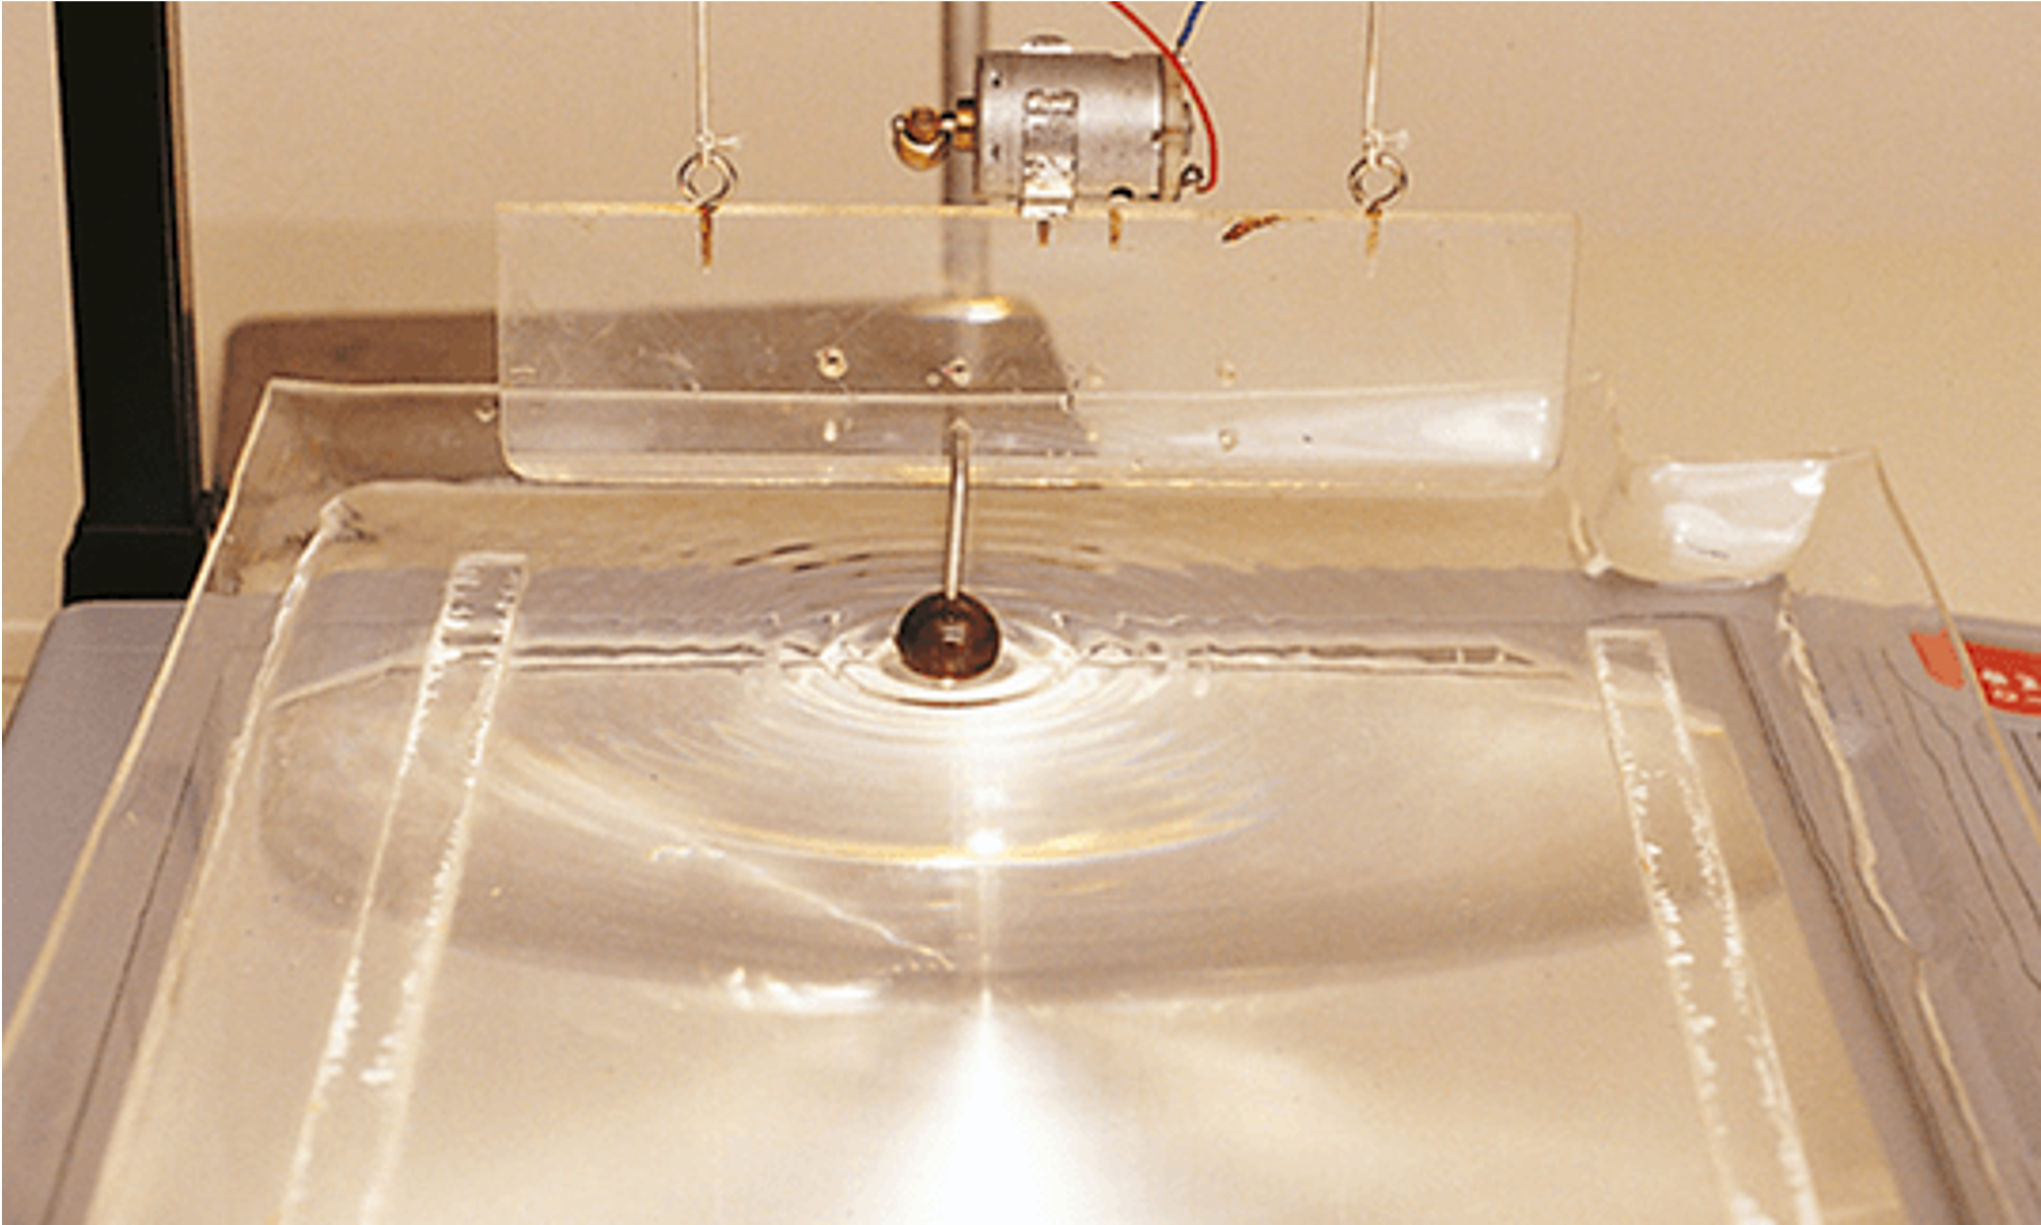
\includegraphics[width=0.4\linewidth]{images/Picture 1.png}
        \caption{週期和距離的關係}

    \end{figure}
\end{frame}

\begin{frame}[t]{例題}
    下圖是相同的繩子在不同時間的情況,求最大的週期和波動對應的移動方向。
    \begin{figure}
        \centering
        \includegraphics[width=0.75\linewidth]{images/Screenshot 2023-09-24 at 10.24.31 PM.png}


    \end{figure}
\end{frame}

\begin{frame}{頻率f}
    \begin{itemize}
        \item 頻率f是質點在一秒內完成多少次循環。
        \item 或是一秒內有多少個完整的波經過某點。
        \item 單位:[Hz]
    \end{itemize}

    \begin{figure}
        \centering
        \includegraphics[width=0.75\linewidth]{images/Screenshot 2023-09-24 at 10.29.53 PM.png}


    \end{figure}
\end{frame}

\begin{frame}{頻率f}
    \begin{itemize}
        \item 在同一個波中,所有質點必須具有相同的頻率。
        \item 頻率的大小僅取決於\textbf{波源}。
    \end{itemize}\bigskip
    \begin{alertblock}{頻率和週期的關係}
        \[f=\frac{1}{T}\]
    \end{alertblock}
\end{frame}

\begin{frame}[t]{例題}
    圖中是一個質點在行波中的\textbf{位移-時間圖}。求波的頻率。
    \begin{figure}
        \centering
        \includegraphics[width=0.75\linewidth]{images/Screenshot 2023-09-24 at 10.40.12 PM.png}


    \end{figure}
\end{frame}
\begin{frame}{例題}
    \begin{figure}
        \centering
        \includegraphics[width=0.6\linewidth]{images/Screenshot 2023-09-24 at 11.04.00 PM.png}


    \end{figure}
\end{frame}
\begin{frame}{波速v}
    \begin{itemize}
        \item 一列波在每單位時間內的傳播距離。
        \item $v=\dfrac{d}{t}$
    \end{itemize}
    \begin{figure}
        \centering
        \includegraphics[width=1\linewidth]{images/Screenshot 2023-09-24 at 10.45.04 PM.png}


    \end{figure}
\end{frame}


\begin{frame}{波速v}
    \begin{itemize}
        \item 對於行波來說:
    \end{itemize}\bigskip
    \input{nodes}
    \bigskip

    \begin{alertblock}{波動方程式}
        \begin{align*}
            v & =\frac{\lambda}{T} \\
            v & =f\lambda
        \end{align*}
    \end{alertblock}
\end{frame}

\begin{frame}{例題}
    \begin{figure}
        \centering
        \includegraphics[width=0.8\linewidth]{images/Screenshot 2023-09-24 at 11.05.21 PM.png}


    \end{figure}
\end{frame}

\begin{frame}{例題}
    \begin{figure}
        \centering
        \includegraphics[width=1\linewidth]{images/Screenshot 2023-09-24 at 11.07.19 PM.png}


    \end{figure}
\end{frame}

\begin{frame}{例題}
    \begin{figure}
        \centering
        \includegraphics[width=0.65\linewidth]{images/Screenshot 2023-09-24 at 11.06.03 PM.png}


    \end{figure}
\end{frame}
\begin{frame}{例題}
    \begin{figure}
        \centering
        \includegraphics[width=0.65\linewidth]{images/Screenshot 2023-09-24 at 11.09.16 PM.png}


    \end{figure}
\end{frame}

\begin{frame}{波速v}
    \begin{itemize}
        \item 波的速度取決於波所傳播的\textbf{介質}。
              \begin{itemize}
                  \item 當波從一個介質傳播到另一個介質時,它的速度會改變。
                  \item 例如:光波在空氣、水和玻璃中會以不同的速度傳播。
              \end{itemize}

    \end{itemize}
\end{frame}

\begin{frame}{影響波速的因素}
    \begin{exampleblock}{水波}
        深水快,淺水慢。
    \end{exampleblock}
    \begin{exampleblock}{繩子上的橫波}
        \begin{itemize}
            \item $\displaystyle v=\sqrt{\frac{T}{\mu}}$
            \item 張力 T$\uparrow \rightarrow$波速$\uparrow$。
            \item 繩子每米的質量 $\mu\uparrow \rightarrow$波速$\downarrow$。
        \end{itemize}
    \end{exampleblock}
    \begin{exampleblock}{聲波}
        波速比較:$v_{\texttt{固體}}>v_{\texttt{液體}}>v_{\texttt{氣體}}$。
    \end{exampleblock}

    \begin{exampleblock}{電磁波}
        折射率 n $\uparrow \rightarrow$波速$\downarrow$。
    \end{exampleblock}

\end{frame}

\begin{frame}{波峰和波谷}
    \begin{itemize}
        \item 最高點:波峰
        \item 最低點:波谷
    \end{itemize}
    \begin{figure}
        \centering
        \includegraphics[width=0.75\linewidth]{images/Screenshot 2023-09-24 at 11.14.35 PM.png}
        \caption{C代表波峰,T代表波谷}

    \end{figure}

\end{frame}

\begin{frame}{波峰和波谷}
    \begin{itemize}
        \item 波峰(波谷)和相鄰波峰(波谷)之間的距離等於一個波長$\lambda$。
        \item 波峰或波谷上位移的量值等於振幅A。
        \item 波峰或波谷上的質點必定是瞬時靜止。
    \end{itemize}
\end{frame}

\begin{frame}{密部和疏部}
    \begin{figure}
        \centering
        \includegraphics[width=0.75\linewidth]{images/Screenshot 2023-09-24 at 11.38.36 PM.png}
        \caption{C代表密部中心,R代表疏部中心}

    \end{figure}
    \begin{itemize}
        \item 密部和疏部\textbf{處於平衡位置}。
        \item 密部(疏部)和相鄰密部(疏部)之間的距離等於一個波長$\lambda$。
        \item 密部和疏部上的質點速率為最大值。
        \item 密部(疏部)和相鄰密部(疏部)中間的質點處於極端位置,其位移等於振幅。
    \end{itemize}
\end{frame}

\begin{frame}{關係線圖}
    \begin{block}{位移-距離圖}
        表示一瞬間各個質點的位移情況。
    \end{block}\bigskip
    \begin{block}{位移-時間圖}
        表示一個質點在不同時間的位移情況。
    \end{block}


\end{frame}

\begin{frame}{}
    \begin{figure}
        \centering
        \includegraphics[width=.8\linewidth]{images/Screenshot 2023-09-24 at 11.59.38 PM.png}


    \end{figure}
    \begin{figure}
        \centering
        \includegraphics[width=.8\linewidth]{images/Screenshot 2023-09-25 at 12.00.57 AM.png}


    \end{figure}
\end{frame}

\begin{frame}{行波}
    \begin{itemize}
        \item 在行波中,每個質點具有相同的能量(KE+PE),和相同的振幅。
        \item 在行波中,波形和能量向前傳播。
        \item 質點只會以平衡位置為中心進行振動。
        \item 質點的移動速率$\neq$行波的速率。
    \end{itemize}
\end{frame}

\begin{frame}[t]{例題}
    \begin{figure}
        \centering
        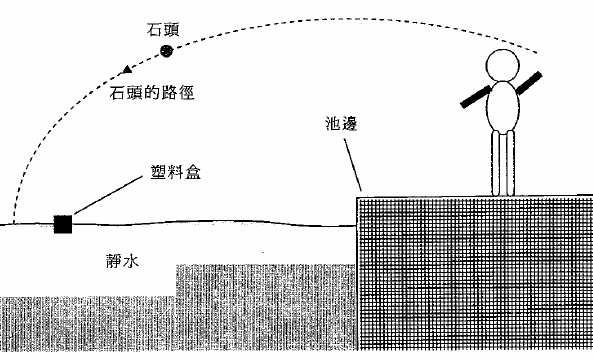
\includegraphics[width=0.5\linewidth]{images/Screenshot 2023-09-25 at 3.02.30 AM.png}


    \end{figure}
    小孩不小心把寶貝盒子掉到海裡了,他試圖用石塊製造出水波把盒子推回來,解釋水波能否將盒子推向池邊。(2分)
    \bigskip
    \begin{itemize}
        \item 不能。波只傳遞能量,不傳遞物質。
        \item 盒子只會在原來位置上下振動。
    \end{itemize}
\end{frame}

\begin{frame}[t]{例題}
    \begin{figure}
        \centering
        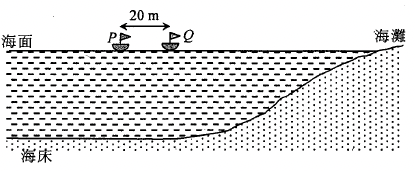
\includegraphics[width=0.6\linewidth]{images/Screenshot 2023-09-25 at 2.56.42 AM.png}


    \end{figure}
    圖中顯示某海灘的切面圖及兩隻小船所在的位置。PQ=20m。現有平直的波浪向着海灘前進。波浪從P運行至Q需時4s。求波浪在P、Q之間運行時的平衡速率。
\end{frame}



\begin{frame}{判斷行波中質點的移動方向}

    \begin{figure}
        \centering
        \includegraphics[width=1\linewidth]{images/Screenshot 2023-09-25 at 12.11.15 AM.png}
        \caption{注意在同一樣波形,各質點的移動方向取決於行波的傳播方向。}

    \end{figure}
\end{frame}

\begin{frame}{判斷行波中質點的移動方向}
    \begin{figure}
        \centering
        \includegraphics[width=0.75\linewidth]{images/Screenshot 2023-09-25 at 12.19.19 AM.png}


    \end{figure}
    \bigskip
    \begin{table}[]
        \begin{tabular}{l|l|l|l|l}
            速率最大 & 速度最大 & 加速度最大   & 動能最大 & 勢能最大 \\
            \hline
                 &      &         &      &      \\
                 &      &         &      &      \\
            \hline
            速率最小 & 速度最小 & 加速度$=0$ & 動能最小 & 勢能最小 \\
            \hline
                 &      &         &      &      \\
                 &      &         &      &      \\
            % \hline
        \end{tabular}
    \end{table}


\end{frame}

\begin{frame}{例題}
    \begin{figure}
        \centering
        \includegraphics[width=0.7\linewidth]{images/Screenshot 2023-09-25 at 12.15.14 AM.png}


    \end{figure}
    \begin{figure}
        \centering
        \includegraphics[width=0.5\linewidth]{images/Screenshot 2023-09-25 at 12.16.00 AM.png}


    \end{figure}
\end{frame}

\begin{frame}{例題}
    \begin{figure}
        \centering
        \includegraphics[width=0.85\linewidth]{images/Screenshot 2023-09-25 at 12.16.42 AM.png}


    \end{figure}
\end{frame}

\begin{frame}{相位}
    \begin{itemize}
        \item 每個質點都有不同的相位。
        \item 兩個距離為 0$\lambda$、1$\lambda$、2$\lambda$、... 的質點屬於\textbf{同相}。
        \item 兩個距離為 $\frac{1}{2}\lambda$、$1\frac{1}{2}\lambda$、$2\frac{1}{2}\lambda$、... 的質點屬於\textbf{反相}。
        \item 不是同相也不是反相的質點屬於\textbf{異相}。
    \end{itemize}
    \begin{figure}
        \centering
        \includegraphics[width=0.75\linewidth]{images/Screenshot 2023-09-25 at 12.41.05 AM.png}


    \end{figure}
\end{frame}
\begin{frame}{相位差}
    \begin{itemize}
        \item 同相的質點之間的距離為為 0$\lambda$、1$\lambda$、2$\lambda$、...,\par 相位差分別為$0(=0^\circ)$、$2\pi(=360^\circ)$、$4\pi(=720^\circ)$、...
        \item 反相的質點之間的距離為為 $\frac{1}{2}\lambda$、$1\frac{1}{2}\lambda$、$2\frac{1}{2}\lambda$、... ,\par 相位差分別為$\pi(=180^\circ)$、$3\pi(=540^\circ)$、$5\pi(=900^\circ)$、...
        \item 同相的質點必定在任何時候以\textbf{相同}方向移動。
        \item 反相的質點必定在任何時候以\textbf{相反}方向移動。
        \item 兩個同相(反相)的質點的速率可以是不一樣。

    \end{itemize}
\end{frame}

\begin{frame}{縱波的位移-距離圖}
    \begin{figure}
        \centering
        \includegraphics[width=0.85\linewidth]{images/longitudinal_graph.png}


    \end{figure}
\end{frame}
\begin{frame}{縱波的位移-距離圖}
    \begin{figure}
        \centering
        \includegraphics[width=1\linewidth]{images/longitudinal_graph_abel.png}


    \end{figure}
\end{frame}

\begin{frame}[t]{例題}
    \begin{figure}
        \centering
        \includegraphics[width=1\linewidth]{images/longitudinal_particles.png}


    \end{figure}
\end{frame}

\begin{frame}[t]{例題}
    \begin{figure}
        \centering
        \includegraphics[width=0.8\linewidth]{images/Screenshot 2023-09-25 at 1.05.49 AM.png}


    \end{figure}
\end{frame}

\begin{frame}{例題}
    \begin{figure}
        \centering
        \includegraphics[width=0.75\linewidth]{images/Screenshot 2023-09-25 at 1.08.39 AM.png}


    \end{figure}
    \begin{figure}
        \centering
        \includegraphics[width=0.6\linewidth]{images/Screenshot 2023-09-25 at 1.09.21 AM.png}


    \end{figure}
\end{frame}

\begin{frame}{例題}
    \begin{figure}
        \centering
        \includegraphics[width=1\linewidth]{images/Screenshot 2023-09-25 at 1.09.58 AM.png}


    \end{figure}
\end{frame}



\end{document}